\documentclass[11pt]{article}
\usepackage{fullpage,amsmath,mathtools, algorithm2e, forest}
\usepackage[mathletters]{ucs}
\usepackage{hyperref}
\usepackage[utf8x]{inputenc}
\usepackage{graphicx}
\usepackage{listings}
\usepackage{courier}

\lstset{basicstyle=\footnotesize\ttfamily,breaklines=true}
\lstset{frame=single}

\graphicspath{ {./images/} }
\title{COMP 4601 - Assignment 2}
\author{Student Name: Brian Ferch\\
\text{Student Number: 100962115}\\\\ 
Student Name: Jules Kuehn\\
\text{Student Number: 100661464}}
\date{Winter 2019}
\begin{document}
\maketitle


\section{Generating user profiles from reviews}

A wealth of metadata was contained within the /reviews/ HTML files. This included:
\begin{itemize}
    \item Movie ID (ex. B0000D0XZ4)
    \item User ID (ex. A1A69DJ2KPU4CH)
    \item User profile name (ex. James Ferguson)
    \item Rating of movie (ex. 5.0)
    \item Review helpfulness (ex. 64/74)
    \item Review time (ex. 1287273600)
\end{itemize}
We scraped all of this data except the review times, although this data has value as well (see "Future work" below). For the purposes of this assignment, the simplification / assumption is that users have static preferences over time.
\newline
While it is certainly possible to do sentiment analysis on the individual reviews (as we have done for the in-class assignment), we felt that given these "true" user ratings, it made more sense to make use of this explicit data than any extracted sentiment. So, the reviews data was processed into the following format:
\begin{itemize}
    \item A "ratings table" where each row label is a User ID, and each column label is a Movie ID. The data contained in this table is the rating of the movie. The rating scale is from 1 to 5, but we stored the values as between 0 and 1, with a value of -1 for a movie not reviewed by this user. The formula for converting star ratings to the range 0 to 1 is $rFloat = \frac{(rStar-1)}{4}$.
    \item A "helpfulness table" corresponding with the same dimensions and labels as above, but storing the helpfulness of each review (parsed to a float)
    \item A map from User ID to User profile name
\end{itemize}
Given this information, some useful characterizations can be made on each user. Included in each of our user profiles is that user's:
\begin{itemize}
    \item Average star rating
    \item Average helpfulness (as rated by other users)
    \item Community affiliation
    \item Position in relation to other users in 2d space
\end{itemize}
% The process by which the community affiliation and 2d representation were obtained is described below.

\section{Clustering users into communities}

The ratings table is large: 1252 rows (users) x 1079 columns (movies). It is also very sparse (93.9\% empty). We first reduced this to a dense, low-dimensional representation by the following process:
\begin{enumerate}
    \item Calculate average ratings for each movie, each user, and the overall average
    \item Fill the missing ratings with the movie's average rating, adjusted to the user's average rating: $rFill = movieAvg + userAvg - overallAvg$
    \item Normalize the matrix to adjust for user average ratings in general.
    \item Determine an appropriate number of dimensions $k$ for truncation.
\end{enumerate}
Reconstructing the original matrix from the 2-dimensional truncated SVD yields an error of 29.2\% without filling or normalization. After filling and normalization though, the error is reduced to 23.7\%. Truncating at 200 dimensions, this error drops to 9.3\%. However, this has little effect on the clustering of users. We can see below that the user clusters determined from the 200-dimensional representation are very similar to the 2-dimensional representation, and that the vast majority of the variance occurs in a single dimension.
\begin{figure}[h!]
    \centering
    \begin{minipage}{0.45\textwidth}
        \centering
        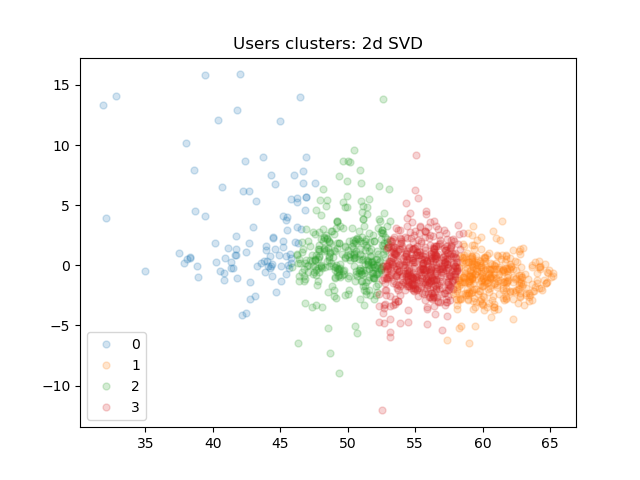
\includegraphics[width=0.9\textwidth]{user_clusters_2d} % first figure itself
        \caption{Kmeans clustering on users in 2d}
    \end{minipage}\hfill
    \begin{minipage}{0.45\textwidth}
        \centering
        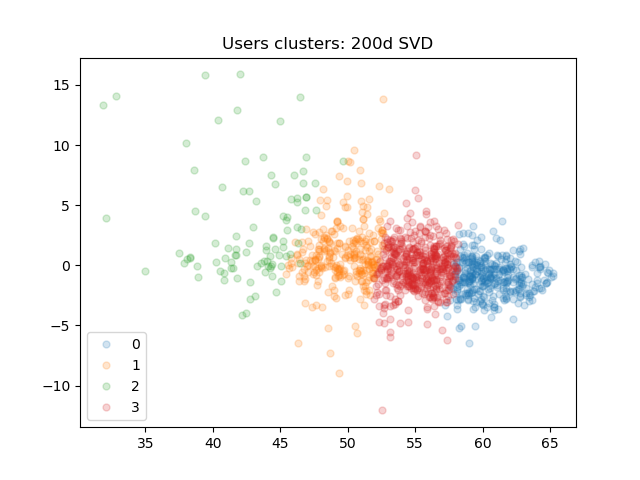
\includegraphics[width=0.9\textwidth]{user_clusters_200d} % second figure itself
        \caption{Very similar results in 200d}
    \end{minipage}
\end{figure}\newline

Given these results, we used a 2-dimensional representation for users. We determined the best number of clusters to be $m = 4$ based on elbow finding in both 2d and 200d. The process ultimately generated two useful mappings: User ID to 2D representation, and User ID to community number.

\begin{figure}[h!]
    \centering
    \begin{minipage}{0.45\textwidth}
        \centering
        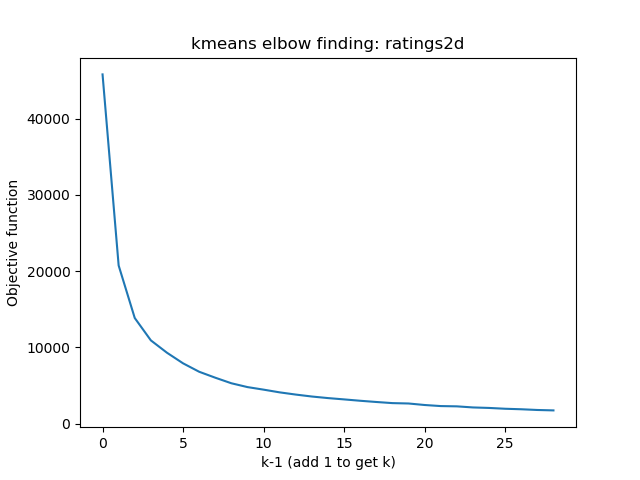
\includegraphics[width=0.9\textwidth]{kmeans_elbow_2d} % first figure itself
        \caption{Suggests 4 clusters of users}
    \end{minipage}\hfill
    \begin{minipage}{0.45\textwidth}
        \centering
        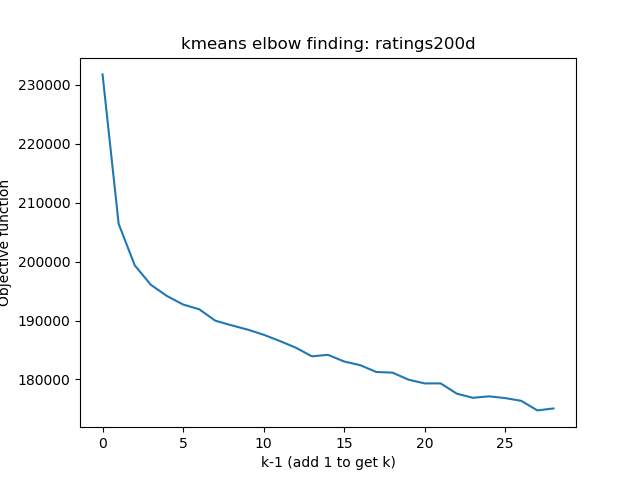
\includegraphics[width=0.9\textwidth]{kmeans_elbow_200d} % second figure itself
        \caption{Similar results in 200d}
    \end{minipage}
\end{figure}\newline


% \lstinputlisting{results/results.txt}

% \begin{figure}[h!]
%     \centering
%      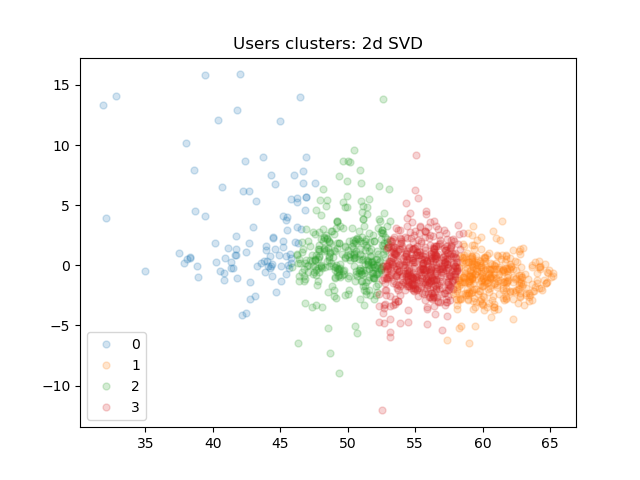
\includegraphics[width=0.5\textwidth]{user_clusters_2d}
%         \caption{Percentage of Recognition Errors}
% \end{figure}

\section{Topic analysis on movies according to page text}

...

\section{Generating and retrieving contextual advertisements}

...

\section{SUGGEST algorithm}

...

\section{Improvements}

...

\end{document}